\section{The xenon normalisation and the relic abundance}\label{sec:lz}

Two conditions anchor the model. The first is the LZ recoil yield, which fixes the combination $\kappa$ of Eq.~\eqref{eq:kappa} as a function of the dark mass. The second is the Planck abundance, which fixes the dark coupling at each mediator mass. Neither condition alone determines the point; together they fix it, and the order in which they are applied fixes which combination is solved first.

\subsection{The recoil normalisation}

At zero momentum transfer the vector current measures the net quark content of the nucleon, so the proton and neutron couplings are $f_p=2g_{Vu}+g_{Vd}$ and $f_n=g_{Vu}+2g_{Vd}$. With the mass-proportional assignment of Eq.~\eqref{eq:lag} this gives $f_p/g_t=5.29\times10^{-5}$ and $f_n/g_t=6.74\times10^{-5}$, and for a xenon nucleus the amplitudes add coherently into the charge $Q_A=Zf_p+(A-Z)f_n$. The differential recoil rate for the exothermic transition is
\begin{equation}
\begin{aligned}
\frac{dR}{dE_R}&=\frac{f_2\,\rho_\chi}{m_2}\sum_A w_A\,
\frac{(g_\chi Q_A/2)^2F_A^2(q)}{2\pi\,(M_V^2+q^2)^2}\;\eta(v_{\min}),\\
v_{\min}&=\frac{|m_AE_R/\mu_A-\Delta m|}{\sqrt{2m_AE_R}},
\end{aligned}
\label{eq:recoil}
\end{equation}
where $w_A$ is the isotopic mass fraction, $F_A(q)$ the Helm nuclear form factor \cite{HELM}, $\mu_A$ the reduced mass, and $\eta(v_{\min})$ the integral of the truncated Maxwell-Boltzmann speed distribution over the local halo. We adopt the benchmark set $v_0=238$~km\,s$^{-1}$, $v_E=254$~km\,s$^{-1}$ and $v_{\rm esc}=544$~km\,s$^{-1}$ with $\rho_\chi=0.3\ \mathrm{GeV\,cm^{-3}}$; the escape speed is the RAVE determination \cite{SHM} and the remaining values are the standard benchmark choices of the direct-detection literature, stated here so that the integral can be reproduced. The energy released by the transition, $\Delta m$, appears only through $v_{\min}$: it lowers the speed required for a given recoil energy and thereby extends the reach of the detector to heavier dark states.

Only the heavier state, $m_2=m_\chi+\Delta m$, can scatter exothermically, so the rate is proportional to its local density, written $f_2\rho_\chi$ in Eq.~\eqref{eq:recoil}, with $\rho_\chi=0.3\ \mathrm{GeV\,cm^{-3}}$ the total local density. We take $f_2=1/2$, the value the two quasi-degenerate states carry while they are in thermal equilibrium at freeze-out, and assume that the ratio survives to the present day. This is an assumption and not a derived result: the splitting is small enough for both states to be populated in the early universe, but a late-time depletion of the excited component would suppress the rate and require a larger $\kappa$, scaling as $f_2^{-1/2}$. Because $\kappa$ is fixed by the same data, the choice of $f_2$ rescales the required coupling, and we state it explicitly so that a reader who adopts another value can rescale the normalisation.

We normalise Eq.~\eqref{eq:recoil} to a reference yield in the LZ region of interest, $N_{\rm ROI}=1.12044$ events. This number is a convention and not a prediction of the present work: it is the integrated rate of a benchmark point over $5.4$--$269.9$~keV nuclear recoil for an exposure of $2.84$~tonne-years, computed at truth level, with no detector efficiency, no energy resolution and no background subtraction, and chosen so that the yield is of the order of the single event reported for the LZ candidate after detector response. Because $N_{\rm ROI}\propto\kappa^{2}$, a different reference yield $N'_{\rm ROI}$ rescales the normalisation as $\kappa'=\kappa\sqrt{N'_{\rm ROI}/N_{\rm ROI}}$, and a different excited-state fraction as $\kappa\propto f_2^{-1/2}$. The normalisation $\kappa(m_\chi)$ is obtained by running the recoil integral at the trial mass itself, so no interpolation table enters the solution and every grid point carries its own value of $\kappa$. Because the recoil rate depends on the couplings and the mediator mass only through $g_\chi^2g_t^2/M_V^4=\kappa^2$, the resulting $\kappa(m_\chi)$, in GeV$^{-2}$, can be combined with any mediator mass through Eq.~\eqref{eq:kappa}. Over the 470 points of the final grid the normalisation takes values $1.18\times10^{-5}\le\kappa\le8.40\times10^{-5}$, and the corresponding dark coupling lies between $0.002$ and $2.28$.

\subsection{The thermal abundance}

The second condition is the Planck abundance \cite{PLANCK}, $\Omega_\chi h^2=0.1200$. For a given $(M_V,g_t)$ we fix $\kappa$ at the trial dark mass through the recoil integral, obtain $g_\chi=\kappa M_V^2/g_t$, and solve
\begin{equation}
\Omega_\chi h^2\big(m_\chi;\,M_V,\,g_t,\,\kappa(m_\chi)\big)=0.1200
\label{eq:relic}
\end{equation}
for $m_\chi$. The equation is solved with \textsc{micrOMEGAs}~\cite{MICROMEGAS} on a logarithmic grid between $8.0$~GeV and $\min(47.8\ \mathrm{GeV},M_V/2)$, with a bisection refinement of the bracketing interval that is run until the residual in $\Omega_\chi h^2$ falls below $10^{-5}$; a root is accepted when $|{\Omega_\chi h^2}/{\rm target}-1|<5\times10^{-3}$. The on-shell requirement $2m_\chi<M_V$ supplies the upper limit wherever it is the tighter of the two; the absolute cap of $47.8$~GeV is the upper end of the mass range over which the recoil normalisation was tabulated~\cite{LZ}, and not a kinematic limit of the model, since the recoil integral remains defined above it. The lower limit of $8$~GeV is where the integral is still defined. Each root is then checked against the two width conditions of Eq.~\eqref{eq:width}.

The model has four parameters, $M_V$, $g_t$, $m_\chi$ and $g_\chi$. The two conditions fix two combinations, so they define a two-dimensional surface rather than a point. We take $(M_V,g_t)$ as the plane and solve for the pair $(m_\chi,g_\chi)$ at each node: the xenon condition fixes $\kappa$ at the trial mass, hence $g_\chi$, and the abundance condition then selects the mass. Every node is an independent solution of the same two equations, and within one mediator-mass column $m_\chi$ varies by a few per cent while $g_\chi$ spans one to two decades.


\subsection{Construction of the physical parameter grid}

Applying the two conditions at fourteen mediator masses between 20 and 200~GeV, and retaining only points that satisfy
\begin{equation}
0<g_\chi\le\sqrt{4\pi},\quad
m_\chi\ge8\ \mathrm{GeV},\quad
\Gamma_V/M_V<0.03,\quad
M_V-m_1-m_2\ge5\Gamma_V,\quad
2m_\chi<M_V,
\label{eq:cuts}
\end{equation}
gives 470 points. Their dark masses lie between 8.42 and 46.59~GeV and their widths satisfy $\Gamma_V/M_V\le2.94\%$; the invisible branching ratio ranges from $1.7\times10^{-5}$ to $1$, the smallest values occurring at the largest couplings of the lightest mediators, where the quark width dominates. The grid is a candidate set for the on-shell branch of the relic solution. Off-shell solutions, which require $2m_\chi>M_V$, are not part of this analysis and are not excluded by it.

Figure~\ref{fig:constraints} shows the solution set in two projections. The left panel places the 470 points in the $(M_V,m_\chi)$ plane, coloured by $g_\chi$, together with the kinematic ceiling $m_\chi=M_V/2$; the dark mass rises with the mediator mass and stays well below the ceiling, so the solutions form a band rather than a diagonal. The right panel shows the same points in the $(m_\chi,g_\chi)$ plane, coloured by $M_V$. Within one mediator-mass column the dark mass changes by at most 8\% (less than 1\% above 90~GeV) while $g_\chi$ spans a factor of 2 to 36, so $M_V$ orders the strips but does not by itself fix either dark parameter.

\begin{figure}[htbp]
\centering
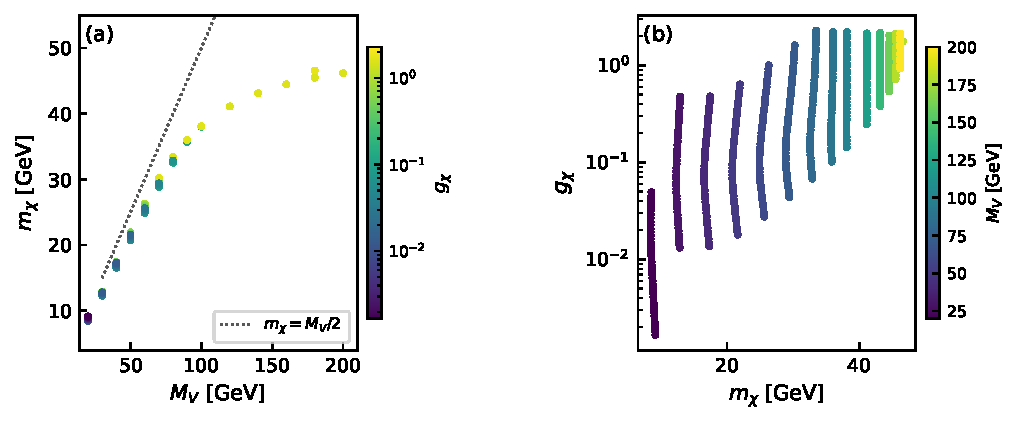
\includegraphics[width=\textwidth]{figs/fig1_v10.pdf}
\caption{The 470 admissible points in two projections. (a) The $(M_V,m_\chi)$ plane, coloured by $g_\chi$, with the kinematic ceiling $m_\chi=M_V/2$. (b) The $(m_\chi,g_\chi)$ plane, coloured by $M_V$. Each vertical strip is one mediator-mass column: $m_\chi$ changes by at most $8\%$ within a column, less than $1\%$ above 90~GeV, while $g_\chi$ spans a factor of 2 to 36.}
\label{fig:constraints}
\end{figure}
